\documentclass[10pt,letterpaper]{article}
\usepackage{spconf,amsmath,amssymb,booktabs,graphicx,microtype,url}
\usepackage[hidelinks]{hyperref}
\title{ParaSeedBench: Wording, Seed, and Finite-Grid Nonadditivity in Text-to-Image Evaluation}
\name{Moshe Laufer$^{1}$, Oren Barkan$^{2}$, Noam Koenigstein$^{1}$}
\address{$^{1}$Tel Aviv University, Tel Aviv, Israel \qquad
$^{2}$The Open University of Israel}
\newcommand{\E}{\mathbb{E}}
\newcommand{\q}{\boldsymbol{q}}
\newcommand{\normk}[1]{\lVert #1\rVert_K^2}
\begin{document}
\maketitle

\begin{abstract}
Text-to-image robustness depends jointly on prompt wording and sampled noise. ParaSeedBench crosses four meaning-equivalent wordings with eight shared seeds and decomposes finite-grid semantic variation into wording, seed, and nonadditive residual components. We evaluate 96 scenes (11,520 images) from three frozen $512\times512$ pipelines and use a prespecified two-rater audit of 1,536 images as primary evidence. Inter-rater joint/atomic agreement is 0.969/0.948. Mean/all-four-wordings accuracy is 0.635/0.414 for PixArt-$\Sigma$, 0.357/0.156 for SD~1.5, and 0.332/0.133 for SDXL. On the same images, automatic scoring underestimates mean accuracy by 0.193, 0.080, and 0.076, respectively. We show that evaluator choice materially shifts measured success and apparent instability, motivating human-primary validation for crossed prompt--seed evaluation. The release provides frozen prompts, seeds, code, provenance, auditable labels, and all 11,520 generated images.
\end{abstract}

\begin{keywords}
text-to-image generation, robustness, semantic evaluation, experimental design, reproducibility
\end{keywords}

\section{Introduction}
Text-to-image (T2I) generators are stochastic systems: an image depends on both a linguistic conditioning signal and sampled noise. Their evaluation should distinguish variation in requested content from permissible variation in unspecified appearance. Given ``a cat left of a dog,'' a change of background is not necessarily an error, but reversing the relation is. Conversely, consistently omitting the dog is stable failure, not reliable generation.

A common diagnostic fixes the seed and compares images generated from equivalent prompts. Another holds the prompt fixed and changes seeds. These comparisons are useful, but neither alone attributes variation exclusively to wording or noise. A generator may react to a wording only for particular initializations. This nonadditivity affects both comparisons. Moreover, equality of output distributions does not imply pointwise equality under a chosen noise coupling: for symmetric $Z$, the variables $Z$ and $-Z$ have identical distributions although paired realizations differ.

We ask: \emph{within a specified prompt--seed grid, how much observed semantic variation is associated with wording, seed, and their nonadditive residual, and how does each coexist with correctness?} ParaSeedBench contributes an auditable crossed evaluation design that jointly attributes finite-grid semantic variation to these components while tracking correctness. It combines an exact descriptive decomposition, controlled prompts, independent human labeling with adjudication, and a checkpointed implementation with explicit provenance and completeness checks. We further show that evaluator choice materially shifts measured success and apparent instability.

\section{Relationship to Prior Evaluation}
TIFA evaluates faithfulness through visual question answering \cite{tifa}; GenEval evaluates compositional object, count, color, and spatial requirements \cite{geneval}. SemVarBench examines responses to linguistic permutations \cite{semvar}. MetaLogic directly tests logically equivalent prompts and diagnoses object, count, and positional inconsistencies \cite{metalogic}. Thus, equivalent-prompt evaluation and these semantic categories are established ideas. Studies of reliable seeds also demonstrate that initialization can affect compositional performance \cite{seeds}.

Unlike reliable-seed studies that characterize or optimize initialization and paraphrase benchmarks that vary language, ParaSeedBench jointly crosses both axes and validates complete-grid outcomes through independent human labeling and adjudication. Its contribution is a \emph{crossed, correctness-aware analysis} of wording, seed, and their nonadditive residual. It uses standard finite-table orthogonal decomposition, not a new analysis-of-variance estimator. GenEval~2 documents evaluator drift \cite{geneval2}, motivating validation of the semantic response grid. We therefore make adjudicated human states primary on a prespecified main subset and retain the automatic evaluator as a secondary diagnostic.

\section{Finite-Grid Semantic Analysis}
\subsection{Experimental unit and correctness}
Scene $c$ specifies $K_c$ binary visual requirements and $J$ equivalent wordings $p_{cj}$. For each model separately,
\begin{equation}
 x_{cjs}=G(p_{cj},z_s),\quad \q^{H}_{cjs},\q^{M}_{cjs}\in\{0,1\}^{K_c}.
\end{equation}
Here $H$ denotes the resolved human state and $M$ the OWLv2/CLIP state. The seed is reset for every call; wordings share a random stream within a model. Matching integer seeds across architectures does not align their latent semantics. Unless superscripted, the equations below apply to either label source; confirmatory semantic results use $H$, while $M$ is secondary. Joint correctness is $A_{cjs}=\prod_k q_{cjsk}$.

Two primary descriptive endpoints are mean accuracy and empirical worst-wording accuracy:
\begin{equation}
 \bar A=\frac{1}{CJS}\sum_{cjs}A_{cjs},\qquad
 R_{\rm emp}=\frac1C\sum_c\min_j\frac1S\sum_s A_{cjs}.
\end{equation}
$R_{\rm emp}$ is the minimum on a finite observed set, not guaranteed robustness. Even if all wordings have the same true success rate, selecting the lowest sample mean induces downward bias. A scene bootstrap does not remove it. As a sensitivity diagnostic, consider all 35 unordered balanced splits of eight seeds. For each split, select every wording tied for lowest training-half accuracy, average their held-out scores, reverse the halves, and then average across splits. This held-out selected-worst score $R_{\rm ho}$ is invariant to wording order and seed ordering, but remains a sensitivity diagnostic rather than an unbiased population minimum. We also report the fraction of seeds for which \emph{all} four wordings are correct; this is a different estimand.

\subsection{Wording, seed, and nonadditivity}
Suppress $c$, define $\normk{v}=K_c^{-1}\sum_k v_k^2$, and let
\begin{align}
 \mu&=\frac1{JS}\sum_{js}\q_{js},&
 a_j&=\frac1S\sum_s\q_{js}-\mu,\nonumber\\
 b_s&=\frac1J\sum_j\q_{js}-\mu,&
 r_{js}&=\q_{js}-\mu-a_j-b_s.
\end{align}
The finite-grid variation components are
\begin{align}
 V_w&=\frac1J\sum_j\normk{a_j},\quad
 V_s=\frac1S\sum_s\normk{b_s},\nonumber\\
 V_{ws}&=\frac1{JS}\sum_{js}\normk{r_{js}}.
\end{align}
Their sum equals total variation:
\begin{equation}
 \frac1{JS}\sum_{js}\normk{\q_{js}-\mu}=V_w+V_s+V_{ws}.
 \label{eq:partition}
\end{equation}
To see this, expand the square. Each row and column mean of $r$ is zero, and $\sum_j a_j=\sum_s b_s=0$; all cross terms vanish. These are exact empirical components, not unbiased population variance estimates. With one image per cell, numerical nondeterminism and judge error cannot be separately estimated as residual noise. For $J=4,S=8$, an iid Bernoulli no-effects reference assigns expected nonconstant-grid shares $3/31$, $7/31$, and $21/31$ to $V_w,V_s,V_{ws}$, respectively, from their ranks. Raw $V_{ws}$ shares therefore reflect the residual's 21 degrees of freedom and are not evidence that a latent interaction dominates noise.

For binary states, normalized Hamming distance equals squared distance under $\normk{\cdot}$. Define $D_w$ as the mean Hamming distance across unordered wording pairs at each seed, and $D_s$ across unordered seed pairs at each wording. The pairwise-distance identity gives
\begin{equation}
 D_w=\frac{2J}{J-1}(V_w+V_{ws}),\qquad
 D_s=\frac{2S}{S-1}(V_s+V_{ws}).
 \label{eq:disagreement}
\end{equation}
Thus the nonadditive residual contributes to both; comparing their raw magnitudes also involves different finite-size factors. All components are first computed per scene, then averaged with equal category weights. Low variation is interpreted jointly with accuracy, never as success on its own.

\begin{figure}[t]
\centering
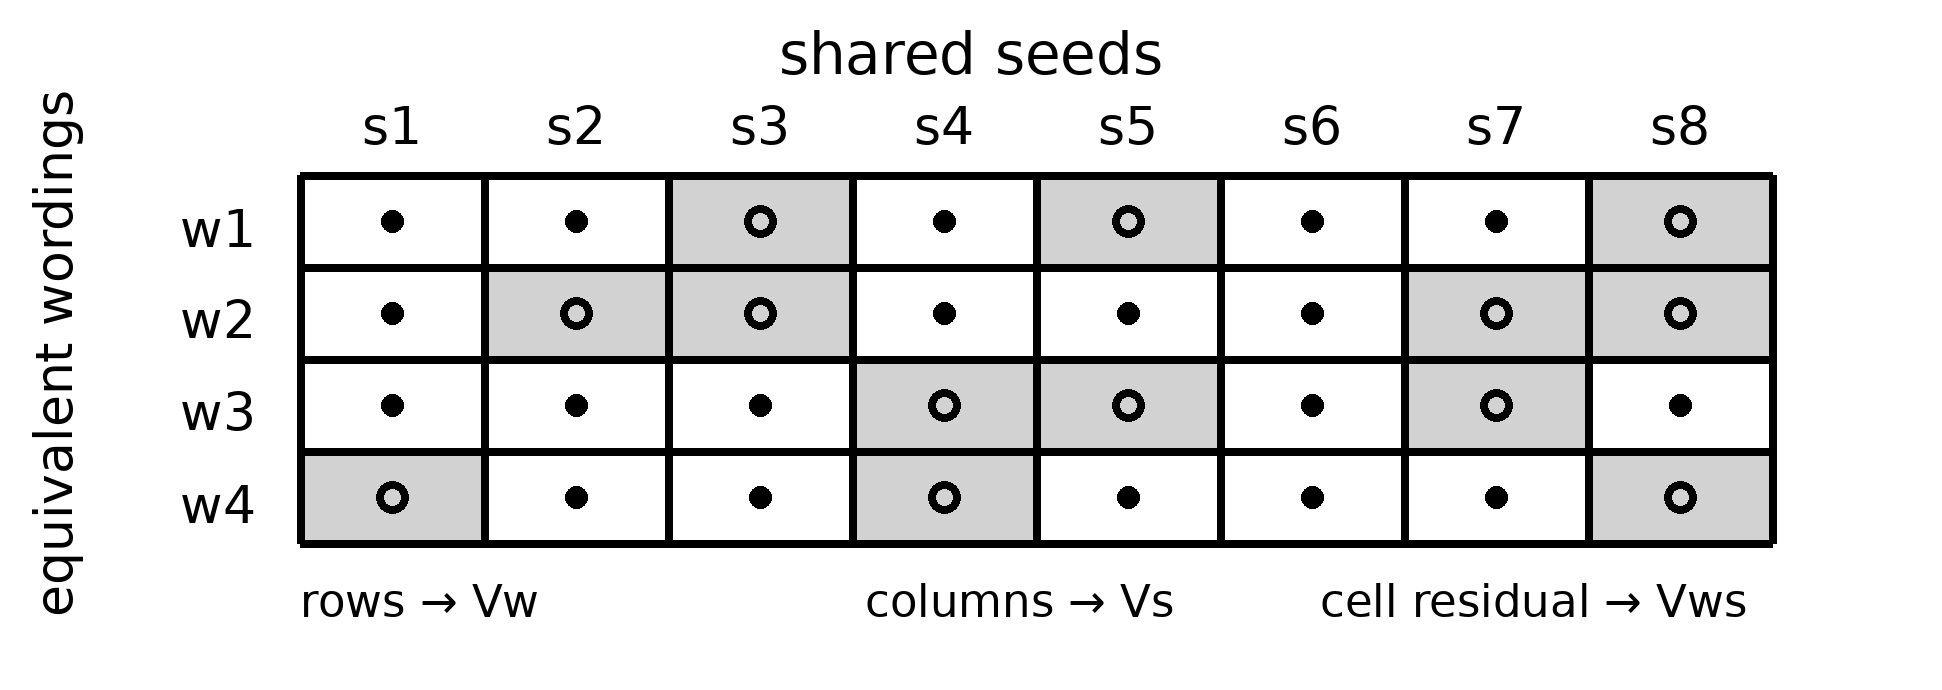
\includegraphics[width=.98\columnwidth]{crossed_grid.png}
\caption{Crossed prompt--seed design (schematic, not model measurements). Rows are four equivalent wordings and columns are eight shared seeds; each cell yields a semantic state $\q_{js}$. Row, column, and cell-specific structure correspond to wording, seed, and nonadditive residual components.}
\label{fig:grid}
\end{figure}

\begin{table}[t]
\centering\caption{Analytical one-atom $2\times2$ examples, not model measurements. Entries of $q$ are arranged as wording rows and seed columns.}
\begin{tabular}{@{}lccccc@{}}\toprule
$q$ & $\bar A$ & $V_w$ & $V_s$ & $V_{ws}$ & $(D_w,D_s)$\\\midrule
$(0,0;0,0)$ & 0 & 0 & 0 & 0 & $(0,0)$\\
$(1,1;1,1)$ & 1 & 0 & 0 & 0 & $(0,0)$\\
$(0,0;1,1)$ & .5 & .25 & 0 & 0 & $(1,0)$\\
$(0,1;1,0)$ & .5 & 0 & 0 & .25 & $(1,1)$\\\bottomrule
\end{tabular}\label{tab:analytical}
\end{table}

\section{Benchmark Protocol}
\subsection{Scenes and data boundaries}
The main suite contains 96 scenes, 24 per category: object existence, exact count, color binding, and spatial relation. Each has four wordings and one meaning-changing control. Scenes use two cyclic pairings over 12 concrete nouns. Counts two, three, and four each appear in eight scenes. All variants request a photograph; spatial paraphrases preserve relative position without introducing sitting or absolute image-edge constraints. Color and spatial prompts explicitly require exactly one instance of each queried object, resolving the evaluator's highest-confidence-instance ambiguity. Other unrequested objects are allowed.

There are 16 separate development scenes using four additional object nouns; a four-scene smoke subset is drawn from these, not from the main set. Main and development semantic specifications are disjoint, including controls. The development audit did not justify evaluator calibration, so thresholds remain declared defaults. Main images did not guide prompts or thresholds. The main prompt set and execution contract were frozen before the completed run; the release preserves the prompt specifications, locked run provenance, and selection manifest.

\subsection{Generators and execution contract}
The controlled $512\times512$ study includes Stable Diffusion~1.5 \cite{ldm}, SDXL-base \cite{sdxl}, and PixArt-$\Sigma$ \cite{pixart}, with respectively 30/30/20 steps and guidance 7.5/7.5/4.5. PixArt uses the 512-MS denoising transformer with the T5, VAE, tokenizer, and scheduler components from its complete 1024-MS Diffusers pipeline; both repository commits are pinned. The scheduler configuration is saved. These settings define the frozen operational pipelines; they are not compute-matched, and SDXL is evaluated below its preferred resolution.

The seed list is $[11,29,47,71,101,131,173,211]$, shared across wordings. A fresh CPU generator is created for every call. FP16 generation, batch size one, disabled TF32, deterministic PyTorch algorithms, fixed negative prompt, and immutable checkpoint commits define the run. PixArt caption cleaning is disabled explicitly. Model-native safety filtering is retained; flagged and all-black outputs are recorded separately and assigned zero correctness for \emph{end-to-end pipeline} accuracy. Rerolling flagged seeds or silently discarding them would change the sampling design.

The main grid contains $96\times5\times8=3840$ images per model, or 11,520 total. The RTX~6000 Ada profile keeps models resident on GPU; the RTX~3070 profile offloads components to CPU. Package versions, source hash, GPU model, CUDA/cuDNN, elapsed generation time, and peak allocated memory are recorded; resumption rejects changed run contracts. A same-process duplicate-input check covers one base scene per category and model.

\subsection{Secondary automatic evaluator and controls}
The evaluator uses OWLv2-base-patch16-ensemble \cite{owlv2} and CLIP ViT-B/32 \cite{clip} in FP32, pinned to immutable revisions. OWLv2 uses an explicitly selected slow processor rather than a version-dependent default. Thresholds 0.10 for detection and 0.35 for class-wise NMS are declared defaults, not validated optima. Color is classified among ten alternatives using the highest-scoring object's box with 3\% padding. Spatial predicates use centroids with a 0.03 image-width/height dead zone. Missing objects fail dependent atoms; exact-one atoms fail when extra queried instances are detected. Correlated detection, color, and boundary errors motivate its secondary status.

For count, color, and spatial controls, evaluate each base/control image against \emph{both} specifications. A paired discrimination success requires each image to satisfy its own specification and fail the alternative. Presence replacement is non-exclusive: an image can satisfy both prompts. It therefore receives own-prompt accuracy but no exclusive-discrimination score. All controls are excluded from the main variation decomposition.

\section{Human-primary Main Results}
\begin{table*}[t]
\centering\small
\caption{Human-primary results on the prespecified 16-scene main audit. Brackets are descriptive 95\% category-stratified scene-bootstrap intervals (2,000 replicates).}
\label{tab:human-primary}
\begin{tabular}{@{}lccc@{}}
\toprule
Metric & PixArt-$\Sigma$ & SDXL & SD 1.5 \\
\midrule
Mean accuracy & 0.635 [0.562, 0.705] & 0.332 [0.287, 0.375] & 0.357 [0.289, 0.418] \\
Empirical worst accuracy & 0.484 [0.422, 0.555] & 0.203 [0.141, 0.258] & 0.234 [0.148, 0.312] \\
All-wordings accuracy & 0.414 [0.344, 0.492] & 0.133 [0.094, 0.172] & 0.156 [0.078, 0.219] \\
Wording disagreement & 0.166 [0.136, 0.198] & 0.265 [0.223, 0.299] & 0.271 [0.227, 0.318] \\
Seed disagreement & 0.204 [0.169, 0.238] & 0.395 [0.365, 0.427] & 0.328 [0.286, 0.373] \\
$V_{ws}$ & 0.052 [0.044, 0.061] & 0.083 [0.071, 0.094] & 0.083 [0.070, 0.096] \\
\bottomrule
\end{tabular}

\end{table*}

\subsection{Resolved two-rater audit}
Using seed 2027, the audit selected four scenes uniformly without replacement within each category, independently of scores. All four equivalent wordings, eight seeds, and three models gave 1,536 images. Two raters independently labeled every semantic atom under neutral identifiers. Both rating interfaces withheld model identity and automatic labels; the adjudication interface also withheld the two prior state vectors, although visual style could still reveal model family. A separate adjudication pass resolved disagreements and was not treated as a third independent rating. Before adjudication, 144 \emph{images} had unequal state vectors, comprising 199 differing atom bits (141 versus 58 in the two directions). Inter-rater atomic agreement was 0.948 with $\kappa=0.891$; joint correctness agreement was 0.969 with $\kappa=0.937$.

Under the frozen $512\times512$ pipelines, Table~\ref{tab:human-primary} gives audited mean accuracy 0.635 for PixArt-$\Sigma$, 0.357 for SD~1.5, and 0.332 for SDXL. Paired scene differences were $+0.277$ [0.197,0.365] for PixArt versus SD~1.5, $+0.303$ [0.232,0.373] for PixArt versus SDXL, and $+0.025$ [$-0.033$,0.084] for SD~1.5 versus SDXL. Stability alone did not imply correctness.

\begin{table}[t]
\centering\small
\caption{Finite-grid variance components. H16 is human-primary on the 16-scene audit; M16 is automatic scoring on the same grids; M96 is automatic scoring on the full 96-scene main suite.}
\label{tab:decomp}
\begin{tabular}{@{}llrrr@{}}\toprule
Scope & Model & $V_w$ & $V_s$ & $V_{ws}$\\\midrule
H16 & PixArt-$\Sigma$ & .010 & .037 & .052\\
H16 & SDXL & .016 & .090 & .083\\
H16 & SD~1.5 & .018 & .061 & .083\\
M16 & PixArt-$\Sigma$ & .012 & .046 & .064\\
M16 & SDXL & .012 & .061 & .072\\
M16 & SD~1.5 & .018 & .056 & .071\\
M96 & PixArt-$\Sigma$ & .014 & .045 & .061\\
M96 & SDXL & .015 & .073 & .072\\
M96 & SD~1.5 & .023 & .058 & .080\\\bottomrule
\end{tabular}
\end{table}

The split-symmetrized human-primary $R_{\rm ho}$ values were 0.580 [0.517,0.655] for PixArt-$\Sigma$, 0.315 [0.245,0.383] for SDXL, and 0.347 [0.248,0.432] for SD~1.5. For the variance components, intervals were: PixArt-$\Sigma$, $V_w$ [.007,.014], $V_s$ [.026,.048], $V_{ws}$ [.044,.061]; SDXL, [.011,.022], [.074,.106], [.071,.094]; and SD~1.5, [.012,.026], [.049,.072], [.070,.096]. Dividing each H16 component by its rank gives, in $10^{-3}$ units, wording/seed/residual estimates of 3.3/5.3/2.5 for PixArt-$\Sigma$, 5.3/12.9/4.0 for SDXL, and 6.0/8.7/4.0 for SD~1.5. The seed estimate was largest for every pipeline; the reported marginal intervals separate it from wording only for SDXL. $V_{ws}$ is the realized nonadditive residual and includes unresolved cell-level variation.

\subsection{Automatic diagnostics and evaluator shift}
On the full 96-scene run, M96 values in Table~\ref{tab:decomp} provide secondary diagnostics. On the audit, machine--human joint accuracy/$\kappa$ was 0.725/0.466 for PixArt-$\Sigma$, 0.850/0.640 for SDXL, and 0.834/0.620 for SD~1.5; atomic accuracy was 0.813, 0.817, and 0.804. Machine-minus-human mean accuracy was $-0.193$, $-0.076$, and $-0.080$, respectively. This generator-dependent error precludes treating M96 as confirmatory ground truth.

Across $72\times8=576$ eligible pairs per model, all four conditions held for 37 PixArt-$\Sigma$, 5 SDXL, and 18 SD~1.5 pairs (0.064, 0.009, and 0.031); this is an end-to-end stress test, not evaluator calibration. Automatic generation retained all model-native safety outcomes: SD~1.5 produced 19 censored/all-black outputs; SDXL and PixArt-$\Sigma$ produced none. Median measured generation times on the RTX~6000 Ada were 0.825, 1.506, and 0.877 s/image for SD~1.5, SDXL, and PixArt-$\Sigma$, respectively.

\section{Limitations and Conclusion}
The study is limited to simple templated photographic compositions, author-designed meaning equivalence, four wording templates, eight seeds, and 16 human-audited scenes. One observation per cell cannot separate latent interaction from residual cell-level variation; human labels retain subjectivity, and category-level joint accuracy is affected by differing numbers of required atoms. Development nouns differ from the main suite, some count controls reproduce another base count, and the three operational pipelines are neither compute-matched nor native-resolution-matched. Bootstrap intervals are descriptive under resampling of the selected scenes, do not cover unseen prompt families or seeds, and do not remove empirical-minimum selection bias; no multiplicity-adjusted hypothesis tests are claimed. These constraints limit population-level and architecture-level interpretation.

ParaSeedBench partitions observed semantic variation on a crossed wording--seed grid while keeping correctness explicit. We show that evaluator choice can materially shift both measured success and apparent instability; accordingly, adjudicated human states are primary evidence and full-suite automatic scoring is a reproducible secondary diagnostic. Code, audited evidence, and a link to the full 11,520-image/results archive are at \url{https://github.com/moshe13269/ParaSeedBench}.

\noindent\textit{AI-use disclosure:} OpenAI ChatGPT assisted with language, \LaTeX{}, and code review; it generated neither human labels nor empirical results, and the authors verified all content.

\clearpage
\ifnum\value{page}=5\relax\else\PackageError{ParaSeedBench}{Technical content must occupy exactly four pages}{Expected permitted page-5 material to begin on page 5.}\fi
\section*{Compliance with Ethical Standards}
Formal ethics review was waived for this minimal-risk annotation study by the responsible institutional ethics committee. The two adult raters voluntarily annotated generated images; no identifying or sensitive personal data were collected. No funding was received for conducting this study. The authors have no relevant financial or nonfinancial interests to disclose.

\begin{thebibliography}{12}
\bibitem{tifa} Y. Hu et al., ``TIFA: Accurate and interpretable text-to-image faithfulness evaluation with question answering,'' in \emph{Proc. ICCV}, 2023.
\bibitem{geneval} D. Ghosh et al., ``GenEval: An object-focused framework for evaluating text-to-image alignment,'' in \emph{Proc. NeurIPS}, 2023.
\bibitem{semvar} X. Zhu et al., ``Evaluating semantic variation in text-to-image synthesis: A causal perspective,'' in \emph{Proc. ICLR}, 2025, arXiv:2410.10291.
\bibitem{metalogic} Y. Shen, Y. Shu, H.-Y. Paik, and Y. Sui, ``MetaLogic: Robustness evaluation of text-to-image models via logically equivalent prompts,'' arXiv:2510.00796, 2025.
\bibitem{seeds} S. Li, H. Le, J. Xu, and M. Salzmann, ``All seeds are not equal: Enhancing compositional text-to-image generation with reliable random seeds,'' in \emph{Proc. ICLR}, 2025, arXiv:2411.18810.
\bibitem{geneval2} A. Kamath et al., ``GenEval 2: Addressing benchmark drift in text-to-image evaluation,'' arXiv:2512.16853, 2025.
\bibitem{ldm} R. Rombach et al., ``High-resolution image synthesis with latent diffusion models,'' in \emph{Proc. CVPR}, 2022.
\bibitem{sdxl} D. Podell et al., ``SDXL: Improving latent diffusion models for high-resolution image synthesis,'' arXiv:2307.01952, 2023.
\bibitem{pixart} J. Chen et al., ``PixArt-$\Sigma$: Weak-to-strong training of diffusion transformer for 4K text-to-image generation,'' arXiv:2403.04692, 2024.
\bibitem{owlv2} M. Minderer, A. Gritsenko, and N. Houlsby, ``Scaling open-vocabulary object detection,'' arXiv:2306.09683, 2023.
\bibitem{clip} A. Radford et al., ``Learning transferable visual models from natural language supervision,'' in \emph{Proc. ICML}, 2021.
\end{thebibliography}
\end{document}
